\section{{\UTP} implementation}
\label{sec:model_implementation}

%%%
% fusion XML
% outil XML > JSON
% PoC : MZN
% Expérimentations
%%%

%The \UTP{} language is a domain-specific language to model a class of university timetabling problems.
%We decided to solve the instances using constraint programming (\CP{}).
In this section, we present the toolchain illustrated in Figure~\ref{fig:toolchain} that is used to process and convert \UTP{} instances to \CP{} compatible formats. We then briefly introduce a generic \CP{} model and its alternative implementation in \MINIZINC{} \cite{MZN} and \CHR{} \cite{Fruhwirth_TechReport_92,Fruhwirth_CP_94,Fruhwirth_JLP_98,Fruhwirth_CHR_09,Fruhwirth_Abdennadher_CHR_03,Fruhwirth_Raiser_2011}. Lastly, we present the experiments carried out on a real instance.

\begin{figure}
    \centering
    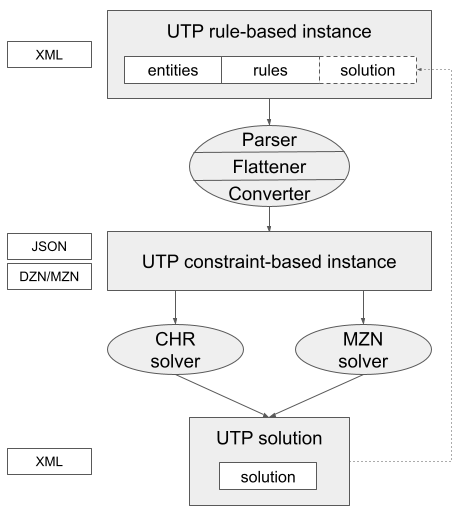
\includegraphics[width=\columnwidth]{2022_APIA/img/utp_toolchain.png}
    \caption{The \UTP{} toolchain}
    \label{fig:toolchain}
\end{figure}

% intro
%The \UTP{} language is easy to describe a timetabling problem instance, but it has to be converted into constraints to be solved.
%We developed a tool that translate a \UTP{} instance into a \CP{} instance.
%We implemented two solvers: one using \MINIZINC{} and one using constraint logic programming with \CHR{}.
%Both solvers were used to solve a real instance.

\subsection{Merger, Parser, Flattener and Converter}
The \UTP{} language is embedded in \XML{}
and comes with a \PHP{} tool 
which combines a parser, a rules flattener and a converter.
The flattener processes rules to generate collections of {\UTP} constraints
and the converter transforms the resulting constraint-based instance into 
\CP{} solver compatible formats based on \JSON{} and \DZN{} (\MINIZINC{} instance format).
%format which may be read by .

The tool also allows to merge \UTP{} instances
into one.
%A \UTP{} instance may thus be built by merging smaller instances
This is useful as data and requirements are usually captured separately for different curriculae or even courses. % and by different stakeholders (e.g., faculty departments, course owners, teachers, etc.).
For instance, one would typically merge all curriculum instances in a faculty. %of individual courses.
% \XML{} files.
%
%The tool was developed in \PHP{} and is available on our website \cite{USPsite}.
%\todo[inline]{Je ne comprends pas la transition (ou l'absence de transition) avec la section suivante. On est d'accord que le "traducteur" XML -> CP-JSON applique ce qui est décrit en 4.2 non ? Dans ce cas, ça manque d'une phrase de liaison (ou alors ce dernier paragraphe devrait être coupé en 2, et mis en partie en 4.2. }
Two \UTP{} instances can be merged as long as they share the same time grid.
All resources (rooms, teachers and students) with the same identifier are merged, e.g. a student may appear in original files and will be present once in the merged files with all its subscribed courses and assigned groups.
Two files with a course sharing the same identifier cannot be merged.
The rule merging raises the question of the labels and the scope of a rule.
Here there are two solutions: either the labels are merged as is, and if two files share the same labels then the rules using the label will apply to all the resources of the merged file with the label ; either the labels are modified to be unique.
%
The current version of the tool does not change labels, thus the user must be careful with the use of labels in files.

% Présenter le modèle PPC
\subsection{\CP{} Model and Solvers}

The \CP{} model of a \UTP{} instance includes instance data, decision variables, built-in constraints of the entity model and constraints generated from the rules set. %using the {\UTP} predicates.
The input data are a transcription of the entity model and include the time grid, the course hierarchy, the set of resources and the various properties of entities and their relations.
The decision variables model the groups chosen for a class and the group, slot, rooms and teachers chosen for each session.

Sectioning constraints partition students into groups based on course registrations, %, i.e., students may not be placed in the same group if they register to different courses.
forbid group sharing between classes of a course part and impose that every student (through its group) attends each part of a course he is registered to.
They also implement the parent relationships between classes and make sure the maximum size of a class is never exceeded by the total headcount of its groups. 

Resource distribution constraints define the domains of resource allocation variables (i.e. allowed rooms and teachers for each session)
and enforce cardinality restrictions regarding the number of teachers needed for each session, the number of sessions taught by each teacher in a course part, whether a room is mandatory in a part, and whether a session is single-room or multi-rooms.

Scheduling constraints define the domains of session scheduling variables (i.e. allowed slots per session),
and ensure sessions do not span over two days and are sequenced based on their rank in each class.
Default cumulative capacity constraints apply to all resources to guarantee each room has sufficient capacity to host its assigned sessions at any one time.
Dedicated constraints handle the particular case of multi-room sessions to make sure 
each room is disjunctive while it is being used,
groups are freely distributed and split over the rooms,
and the cumulated capacity of the rooms is considered for hosting.

Lastly, each {\UTP} predicate has a custom constraint-based implementation to achieve the desired semantics.



As a proof of concept, we implemented a {\CP} model for the class of {\UTP} problems using \MINIZINC{} and running {\GECODE} \cite{GECODE} as a back-end solver.
This model makes use of global constraints, notably constraint \texttt{cumulative} \cite{beldiceanu2002new} which serves to handle both cumulative and disjunctive resources.
We implemented a second solver using constraint logic programming in \CHR\ (Constraint Handling Rules) in order to take advantage of the propagation of constraints on variable domains as in \CP\ but also of the global structure of the problem (\CHR\ allows to manipulate symbolic expressions and not only domains).
We used \CHRPP\ \cite{barichard_stephan_2019} to implement the model and solve the instances.



\subsection{Experiments}
We carried out experiments on a real-life instance modeling the second semester of the last year of Bachelor in Computer Sciences at Université d'Angers (available at \cite{USPsite}).

The instance consists of 5 mandatory courses and 2 optional courses to choose amongst 4, 24 course parts and 42 classes, 67 students pre-divided into 4 groups, 12 teachers and 8 rooms.
The time grid is decomposed into 12 weeks, 5 weekdays and 1440 daily slots.
Note that courses last 80 minutes in this Faculty and must be placed on a specific time grid ranging from 08\string:00am to 07\string:50pm with session starting every 90 minutes to account for breaks.
The instance includes 46 rules, namely, 13 constraints \texttt{\WEEKLY}, 16 \texttt{\SEQUENCED}, 2 \texttt{\SAMESLOT}, 5 \texttt{\SAMEWEEK}, 5 \texttt{\SAMEROOMS} and 5 \texttt{\SAMETEACHERS}.

Both \MINIZINC{} and \CHRPP{} solvers were run with an Intel Core i7-10875H 2.30GHz and solved the instance in less than 5 seconds.
%
Source codes for the \MINIZINC{} and \CHRPP{} models are available on our website \cite{USPsite}.